\documentclass[output=paper]{LSP/langsci}
\ChapterDOI{10.5281/zenodo.1090968}

\defcitealias{BBAW2010}{BBAW 2010}

% Article Metadata
\title{Changes of word class during translation -- Insights from a combined analysis of corpus, keystroke logging and eye-tracking data}
\author{Tatiana Serbina\and Sven Hintzen\and Paula Niemietz\lastand Stella Neumann\affiliation{RWTH Aachen University}}
% Abstract
\abstract{%
Drawing upon the data collected in a translation experiment, this study combines product- and process-based analyses of translations with a focus on word class shifts. The keystroke logged translation corpus used in the paper consists not only of source and target texts, but also of the corresponding log files of the translation process data. Thus, in addition to the analyses of the final translation products, this corpus allows us to study changes of word class in the intermediate versions present during the translation process. We also use the complementary eye-tracking data to test our initial assumptions about the cognitive processing associated with nouns, verbs and shifts between these two word classes.}
\rohead{\thechapter\hspace{0.5em}Changes of word class during translation}
\begin{document}
\maketitle
%Section 1
\section{Introduction}\label{serbinaetal:sec:1}
Over the last decades, laboratory experiments have been increasingly employed in translation studies to investigate research questions related to the \isi{translation process} (for an overview see e.g. \citealt{Gopferich2008}). In addition, a number of studies have shown that a combination of process- and product-based analyses of the data collected during such experiments may provide new insights into the nature of translations, for instance by treating keystroke logs as a corpus \citep{Alves2004, Alves:2009js, Alves2011On, Serbina2015Development, Serbina2015Part}. Keystroke logging data contains all the keystrokes and mouse movements produced while writing on a computer. This information can be linked to eye-tracking data to establish not only what an experiment participant was typing but also what stretches of text s/he was looking at \citep{Carl2009}. In purely process-based analyses, this type of data is often studied by comparing writing and reading behavior of individual participants on a rather global level, i.e. the source texts and the produced translations are analyzed with a fairly general look at linguistic phenomena (e.g. \citealt{Dragsted2008}, \citealt{Pavlovic2009}, \citealt{Jensen2011a}). A corpus perspective on the keystroke logs, which are enriched with linguistic annotation and alignment between source and target texts, allows for systematic querying and subsequent quantitative as well as qualitative analyses of linguistic phenomena as they occur in translations across multiple participants. The present study aims at investigating \isi{word class} shifts in translations using a keystroke logged translation corpus \citep{Serbina2015Development}. As discussed in \sectref{serbinaetal:sec:2}, \isi{word class} shifts could be indicative of deeper changes between source and target texts. Focusing on the word classes of nouns and verbs, our analyses take into account not only translation shifts between originals and the final translation products but also changes visible in the numerous intermediate versions, which are variants of the produced text identified at different points during the \isi{translation process}. Including the intermediate versions allows us to also examine changes that occur within the intermediate versions but are discarded in the final translation, information that adds to our understanding of potential causes of these shifts, their existence having been shown in exploratory analyses of \isi{keystroke logging} data (e.g. \citealt{Alves2010}). This makes it possible to perform more detailed analyses of the \isi{word class} shifts. The eye-tracking data adds information that is used to infer the amount of \isi{cognitive effort} involved in such linguistic changes. The analyses draw on the \isi{word class} or part of speech annotation and word level alignment available in our corpus. 
The remainder of the paper is structured as follows. An overview of the theoretical background relevant for the present study is given in \sectref{serbinaetal:sec:2}, and \sectref{serbinaetal:sec:3} introduces the methodology for obtaining the experimental data analyzed in this paper. \sectref{serbinaetal:sec:4} and \sectref{serbinaetal:sec:5} describe the results, related both to the traditional corpus analyses of shifts between source and target texts (\sectref{serbinaetal:sec:4}) and also to additional investigations which can be conducted only with the corpus containing \isi{translation process} data (\sectref{serbinaetal:sec:5}). \sectref{serbinaetal:sec:6} contains concluding remarks and an outlook on further research. 

%Section 2
\section{Theoretical background}\label{serbinaetal:sec:2}
The analysis of translation shifts, i.e. departures from a direct or \isi{literal translation}, is a long-standing research topic in translation studies (cf. \citet{Cyrus2009} for a recent state of the art). Changes in the grammatical category of individual word tokens are referred to as grammatical shift \citep{Catford1965} or transposition \citep{Vinay1995}. A typical example of a change in grammatical category is the change in \isi{word class}, as in example \REF{serbinaetal:ex:1} where the verb \textit{behaves} is translated by the noun \textit{Verhaltensweise} (`behavior-way'). Both items share an equivalent lexical base (\{behav\} and \{verhalt\}).

\ea\label{serbinaetal:ex:1}
\textbf{EO:} Crumpling a sheet of paper seems simple and doesn't require much effort, but explaining why the crumpled ball [behaves] the way it does is another matter entirely. \\
\textbf{GTrans:} Ein Blatt Papier zusammen zu knüllen, erscheint einfach und erfordert wenig Anstrengung; die [Verhaltensweise] des Papierknäuels zu erklären, ist dagegen eine völlig andere Sache. (KLTC PROBRAL GT7\footnote{In all examples taken from the analyzed translation experiment, we use the following notation: KLTC - Keystroke logged translation corpus, GT1-GT8 - experiment participants from the group of \ili{German} professional translators, GP1-GP8 - experiment participants from the group of \ili{German} physicists, EO - English original, GTrans\_i - an intermediate version of the \ili{German} translation, GTrans - the final version of the \ili{German} translation.})
\z

\citet{Vinay1995} and \citet{Newmark1988} approach such shifts from the point of view of procedures (to be) used by the translator in those cases where a direct translation is not desirable or otherwise impossible. At the same time, the investigation of translation shifts is also adopted in descriptive analyses of translation corpora with respect to differences between source and target texts (e.g. \citealt{Cyrus2006}, \citealt{Culo2008}). What these studies have in common is that linguistic units are examined more or less in isolation (with the exception of Cyrus who analyses predicate-argument structures). In contrast, \citet{Steiner2001Translations} suggests that there is systematicity in which shifts occur in which direction by linking some high-level assumptions about typological differences between English and \ili{German} to expected shifts in \isi{word class}. More specifically, he links Hawkins' \citeyearpar{Hawkins1986} idea of a more direct mapping of semantics on grammar in \ili{German} as opposed to English with the systemic functional notion of grammatical \isi{metaphor} (see below), and comes to the conclusion that translators will tend to go for a closer match between semantics and grammar in the translation direction English to \ili{German} by reducing the level of grammatical \isi{metaphoricity}, which is then observable, for instance, in the form of shifts from nouns to verbs. While this hypothesis clearly has some appeal, \citet{Culo2008} report results of transposition in aligned word pairs from the CroCo Corpus \citep{HansenSchirra2012Cross} which run counter to Steiner's hypothesis. Although they do report a proportion of noun to verb shifts of almost 5\% of all transpositions in the translation direction English to \ili{German} in one of the eight CroCo registers, shifts from verbs to nouns account for roughly 24\% of the transpositions. 

One factor potentially explaining this discrepancy between Steiner's hypothesis and the actual frequencies is that Steiner did not take into account the actual distribution of word classes in English and \ili{German}. In his overview of the distributions in the CroCo Corpus, the \ili{German} part of the corpus is reported to have more nominal word classes, whereas English has more verbal word classes \citep[80]{Steiner2012}. Overall, Steiner concludes that nominal word classes including nouns, pronouns, adjectives and adpositions account for a slightly higher share of word classes in the \ili{German} subcorpus in comparison with the English subcorpus than verbal word classes (verbs, adverbs and conjunctions), where the proportions are reversed. The relationship also applies to verbs only. As to nouns, Steiner reports somewhat lower percentages in the \ili{German} than in the English subcorpora. However, divergences in spelling conventions were not taken into consideration in Steiner's analysis. These do not affect the verb count, but have an effect on nouns. While compounds in \ili{German} are usually written as single word tokens which also appear as single tokens in the automatic tokenization, compounds in English are usually written as separate tokens and are hence also tokenized, tagged and counted separately. This well-known difference leads to skewed counts where a compound in English is counted as two word tokens, while its equivalent in \ili{German} is counted as just one token even though it may consist of equivalent individual nouns. 

A cursory look at aligned nouns in the CroCo Corpus (see \tabref{serbinaetal:tab:1}) shows that in most cases the English translation consists of at least one more token.

\begin{table} % "word token count" in table header changed to "Tokens" to fit the page  
\fittable{
    \begin{tabular}{rlrlr}
	\lsptoprule
	No. & \ili{German}  & Tokens & English translation & Tokens\\ 
     \midrule
	1 & Soziale Marktwirtschaft & 2 & social market economy & 3\\
	2 & Systemwechsel & 1 & system change & 2\\
	3 & Fremdsprachenkenntnisse & 1 & knowledge of foreign languages & 4\\
	4 & Aufzugtür & 1 & lift door & 2\\
	5 & Fallhöhe & 1 & depth of the fall & 4\\
	6 & Innenstadt & 1 & city center & 2\\
	7 & Haarnetz & 1 & hairnet & 1\\
	8 & Kaschmirpullover & 1 & cashmere sweater & 2\\
	\lspbottomrule
	\end{tabular}
	}
  	\caption{Equivalents of German compounds from the CroCo Corpus}
  	\label{serbinaetal:tab:1}
\end{table}

\largerpage%longdistance
The higher proportion of nouns in the English subcorpus can, therefore, partly be accounted for by differences in spelling conventions. However, there is no simple computational solution to this problem: The linguistically soundest way to making English and \ili{German} compounds comparable would be to identify those English compounds spelled as separate words and count them as one word token. However, this task is far from straightforward both linguistically -- \citet[589]{Biber1999} call the distinction between phrases and compounds a cline -- and computationally, as there is not all that much systematicity even in the spelling conventions. A search for \textit{hairnet}, \textit{hair net} and \textit{hair-net} in the COCA Corpus \citep[ongoing]{Davies2008}, for instance, retrieves 74 hits for the single token, 31 for the version spelled as two tokens and one hit for the hyphenated compound. In contrast, the query for all three spellings of \textit{city center} retrieves 62 hits for the single token spelling, 628 hits for the two tokens version and 15 hits for the hyphenated spelling. While we may safely assume the hyphenated spelling to occur with consistently lower frequencies, single word and two word spellings appear to alternate. The computational handling of multiword expressions in English is a longstanding issue that continues to receive much attention.\footnote{The Association for Computational Linguistics maintains its own Special Interest Group on Multiword Expressions. For an overview see \citet{Sag2002}, who tellingly entitle their paper ``Multiword Expressions: A pain in the neck for NLP''.} An alternative and more feasible approach is to chunk compounds into individual word tokens, i.e. to make \ili{German} more similar to English. However, this, too, is not entirely unproblematic because some compound nouns are lexicalized. Thus chunking them into their component parts would also break the compound's meaning (see \figref{serbinaetal:fig:1}, where e.g. corpus position 223044, i.e. \textit{Fußgängerbrücke} `pedestrian bridge', displays a potential case of lexicalization whose chunking may be disputed). It therefore makes sense to accept the limitations of the naïve noun count based on automatic tokenization. Nevertheless, this naïve count could be enriched with additional counts to give at least an estimate of the skew introduced by the diverging spelling conventions. For the purpose of this paper we therefore counted compound chunking and noun-noun sequences in the CroCo Corpus. 

In addition to part of speech tagging in both languages\footnote{All analyses of word classes discussed here are based on automatic part of speech tagging \citep{HansenSchirra2012Corpus}. The annotation categories will possibly differ in their conceptualization across languages. The advantage of this language-internal tagging is that the annotation is adapted to (or, in technical terms, trained on) the characteristics of the respective language. As a consequence, the results reflect the contrastive differences between the languages -- provided the automatic tagging is correct. For estimates of the tagger accuracy across the CroCo registers see \citet[50-52]{HansenSchirra2012Corpus}}, the annotation of the CroCo Corpus includes compound chunking as part of the morphology annotation \citep{HansenSchirra2012Corpus}. We queried 110 English original texts and their matching \ili{German} translations, and 121 \ili{German} original texts and their English translations from eight registers for the number of noun tokens containing chunking in the morphology annotation. As can be seen from the selected query hits in \figref{serbinaetal:fig:1}, the query retrieves quite a number of relevant hits as well as cases which would not lead to a higher count of nouns because the compounded element is not a noun (e.g. corpus positions 670, 1144, 223049).\footnote{Compound chunking after the slash is represented by lexical bases separated by hashes.} It also becomes clear that not all chunked word tokens are limited to just one additional noun, thus increasing the number of nouns by more than one (e.g. corpus positions 325, 898). 

\begin{figure}
{\footnotesize
\begin{tabular}{r l}
100:&  <Systemwechsels/system\#wechsel> \\
223:&  <Exportweltmeisterschaft/exportieren\#welt\#meisterschaft> \\
260:&  <Erfolgsgeschichte/erfolg\#geschichte> \\
304:&  <Wörterbuch/wort\#buch> \\
317:&  <Mittelstand/mittel\#stand> \\
325:&  <Beitragsbemessungsgrenze/beitrag\#bemessung\#grenze> \\
328:&  <Superstar/super\#star> \\
618:&  <Geistesblitz/geist\#blitz> \\
670:&  <Solidargemeinschaft/solidarisch\#gemeinschaft> \\
898:&  <Bundeskartellamt/bund\#kartell\#amt> \\
926:&  <Produktivitätspeitsche/produktivität\#peitsche> \\
1084:&  <Nachtwächterstaat/nacht\#wächter\#staat> \\
1144:&  <Rundumversorgung/rundum\#versorgung> \\
222710:&  <Schweizertal/schweizer\#tal> \\
222729:&  <Kaiser-Wilhelm-Denkmal/kaiser\#Wilhelm\#denkmal> \\
222838:&  <Bergbaumuseum/berg\#bau\#museum> \\
222962:&  <Lahn-Uferpromenade/Lahn\#ufer\#promenade> \\
223044:&  <Fußgängerbrücke/fuß\#gänger\#brücke> \\
223049:&  <Experimentierfreude/experimentieren\#freude> 
\end{tabular}}
\caption{Selected query hits of noun tokens containing chunking in the morphology annotation}
\label{serbinaetal:fig:1}
\end{figure}

The results summarized in \tabref{serbinaetal:tab:2} can therefore only provide a rough indication of the differences between English and \ili{German}. Moreover, it is well possible that the automatic morphology annotation with MPRO \citet{Maas1998} reaches different degrees of precision and recall in the two languages. 

\begin{table}
	\centering
	\begin{tabularx}{\textwidth}{lXXXX} 
    \lsptoprule
    					& verbs & nouns & compound nouns& noun-noun sequences 	\\ \midrule
	English originals 	& 14.97 & 26.66 &  0.13 		& 4.63					\\
	\ili{German} originals 	& 11.97 & 24.10 &  6.33 		& 1.58					\\
	English translations& 14.16 & 25.72 &  0.11 		& 4.36					\\
	\ili{German} translations & 12.58 & 24.77 &  5.28 		& 1.77					\\
	\lspbottomrule
	\end{tabularx}
	\caption{Mean frequencies of verbs, nouns, compounds and noun-noun sequences in the texts of the CroCo Corpus reported as percentages of all tokens}
    \label{serbinaetal:tab:2}
\end{table}

The percentage of verb part-of-speech tags displayed in \tabref{serbinaetal:tab:2} is in line with the numbers of \citet{Steiner2012}. The Fisher's exact test performed on the raw frequencies of verbs in the English and \ili{German} originals cross-tabulated with all other word classes shows that the English original texts have significantly more verbs $(42,746 / 243,475)$ than the \ili{German} texts $(35, 471 / 253,019; p < .001, df=1)$. This is partly to be explained by the reliance of English on non-finite subordination, which is not of equal importance in \ili{German} (see \citet{Konigs2011} for a collection of examples). The noun counts in \tabref{serbinaetal:tab:2} seem to paint a different picture. \ili{German} original texts have a lower percentage of nouns than the English original texts. However, the number of compounds shows a clear, but unsurprising tendency of the \ili{German} texts to rely more on nominal expressions than the percentage of nouns alone suggests. The share of noun-noun compounds spelled as one word actually increases the noun count, because each true noun-noun compound consists of (at least) two nouns\footnote{Although the CroCo Corpus contains morphology annotation, which includes the compound chunking discussed in connection with \figref{serbinaetal:fig:1}, the chunked items are not annotated for part-of speech and are thus not included in this count.}. Moreover, noun-noun sequences written as separate words will partly represent compounds, at least in English. While they do not increase the percentage of nouns, because each tokenized word tagged as a noun is already included in the percentage, their relative frequency provides an indication of the role they play in each language and hence facilitates a better estimate of the underlying distribution of nouns.  

Even if we distrust the frequency of compounds and assume that half of the hits are combinations of the head noun with some other \isi{word class} and that there are no combinations of more than two nouns in the compounds, there is still a slightly higher frequency of nouns in \ili{German} (24.10\% plus at least 3\% of compound nouns) than in English (26.66\% plus less than 0.1\%). Additionally, and again being conservative, at least some of the noun-noun sequences will probably represent compounds that would be written as one token in \ili{German} and therefore would reduce the overall number of nouns in English. 

To sum up, the results suggest that \ili{German} not only has a lower frequency of verbs but also a higher frequency of nouns. The analysis is further strengthened by Steiner's analysis of nominal versus verbal parts-of-speech referred to above. In an explorative study of the CroCo corpus, \citet[80]{Steiner2012} suggests that while \ili{German} in total appears to have a higher percentage of nominal parts-of-speech (51.58\% versus 49.72\%), English is characterized as having a higher percentage of verbal parts-of-speech (24.27\% versus 21.64\%). These results also corroborate Čulo et al.'s \citeyearpar{Culo2008} findings based on the analysis of aligned pairs, which showed that there is a directionality effect in shifts in \isi{word class}. According to their results, more verbs are changed into nouns in the translation direction English to \ili{German}, whereas the opposite is the case in the translation direction \ili{German} to English. 

At this stage the counts for translations are included in \tabref{serbinaetal:tab:2} because they will be of use in generating hypotheses and understanding the results of our analyses in \sectref{serbinaetal:sec:4} and \sectref{serbinaetal:sec:5}. Suffice it to say that the translations in both directions show a clear \isi{target language} orientation, albeit to a somewhat reduced extent, thus reflecting some \isi{source language} shining through \citep{Teich2003}. We would claim that based on the frequencies reported above, the longstanding assumption that \ili{German} tends to be more nominal than English is corroborated. This is further complemented by the lower frequency of verbs in \ili{German} which in itself suggests a different relationship between nominal and verbal word classes in the two languages. It is safe to hypothesize on the basis of these different analyses of the CroCo Corpus that translators are guided by the usage-based contrastive differences and tend to make their translations of the source texts more nominal in the translation direction English to \ili{German}.

At the same time, changes between nouns and verbs are in fact only a symptom of a more complex structural change as in \REF{serbinaetal:ex:1}  where the clausal modification is translated by a noun phrase. A translation closer to the original could have been [\ldots] \textit{aber zu erklären, warum sich das Papierknäuel so verhält, wie es das tut,} [\ldots]. The nominal translation is clearly shorter (only three word tokens) and also appears less complex on the level of clause. But condensing the event described in the original to just the noun \textit{Verhaltensweise}, a noun which then also implies a certain temporal extension of an ongoing process, results in a reduced amount of explicit information \citep{Steiner2005, Halliday1999}. In Systemic Functional Linguistics this phenomenon is called grammatical \isi{metaphor}, a mismatch between the grammatical realization and the respective semantic structure of an event, hence the use of the notion of \isi{metaphor} \citep[665]{Halliday2013}. Unlike other related notions, such as transcategorization, it goes beyond simple observations about changes in \isi{word class} by taking into account the wider grammatical and semantic context affected by such changes. It is this richer notion which we use to explain how certain nominal contexts, especially contexts involving nominalization of ongoing events (i.e. process nouns, cf. \citealt{Fontaine2017}), can be described as more complex: they imply more semantic material which, in the explicit counterpart, would have to be expressed by a more complex grammatical structure. However, it should be mentioned that the question of how complexity actually manifests in grammatical structure is far from straightforward. In fact, it manifests at different levels with complexity at one level often being complemented by simple structures at another level. A higher number of verbs leads to increased complexity at the level of the clause because each verb requires satisfying its valency. This often goes hand in hand with reduced complexity at the phrasal level. By contrast, packaging the same meaning into nominal structures will lead to increased complexity at the phrase level with the elements associated with the valency of the nominalized verb being integrated into the noun phrase as modifiers (see, e.g., \citealt{Halliday2001}) or being unmentioned and thus implicit. This, in turn, often goes hand in hand with a simpler clause structure. One might claim that a nominalized noun (or more generally a process noun) itself appears simple enough and is definitely shorter than its clausal counterpart, thus leading to reduced processing effort. However, nominalizations, especially if packaged into grammatically complex nominal structures, are further removed from what might be described as our experience of the world, in which we tend to observe or experience events, rather than entities \citep{Halliday2013}. Consequently, grammatical structures which are more congruent with our experience of the world might be easier to process. In other words, we assume that \isi{metaphoricity} in this sense requires more effort in decoding the combined grammatical and semantic structure (\citealt[15]{Steiner2001Translations}, \citealt[258]{HansenSchirra2012Towards}). Although \citet[260]{HansenSchirra2012Towards} acknowledge ``complete avoidance of unpacking in cases of highly routinized stretches of text which allow direct transfer'' (see also \citealt[145]{Hansen2003The} and \citealt[411]{TirkkonenCondit2005}), their and Steiner's  \citeyearpar{Steiner2001Translations} main assumption is that unpacking the complex grammatical structure is the default and that re-packaging of this structure ``is cut short below the degree [of grammatical \isi{metaphoricity}] to which it might otherwise go'' (\citealt[260]{HansenSchirra2012Towards}). 

To specify our assumptions: in general, we might hypothesize that the translator will avoid increased effort. Complex features are expected to impose higher processing demands during translating as reflected in increased fixation durations etc. on the respective source text segments, longer \isi{pauses} in \isi{text production}, etc. As noted above, we assume that grammatically metaphorical variants involving semantic complexity in combination with syntactic complexity on the level of nominal phrases are more difficult to process than their more congruent versions, even though the latter are still characterized by syntactic complexity on the level of clause. Furthermore, we assume that the reduction of semantic and phrasal complexity is more frequent in translation than its increase because, again, the latter is more effortful. On these grounds, it appears plausible to assume that indicators of increased \isi{cognitive effort} triggered by complexity associated with grammatical \isi{metaphor} can be correlated with reduced complexity in the product. Note that this does not imply that reduction is \textit{more} probable than maintaining the level of complexity. 

\largerpage
Classical approaches to translation shifts do not take into account specific claims about the exact conditions under which a certain shift is more likely to occur. Possible factors affecting the likelihood of the translator opting out of the direct translation are contrastive differences like the ones discussed above, which need to be acted upon either because the feature of the source text is altogether ungrammatical in the \isi{target language} or because the translator is (possibly unconsciously) aware of a \isi{target language} norm and adapts to it (for corpus findings on norm-conforming behavior see \citealt{Delaere2015}). Alternatively processing-related factors such as lack of understanding (also of the just mentioned norms), fatigue and \isi{time pressure} \citep{Steiner2001Translations} may play a role in this variation.\footnote{Note that these factors only make sense when looking at the local context of the immediate \isi{translation process} in which a translation problem occurs. All of these are liable to being further modified (i) to ensure overall cohesion and coherence of the translation and (ii) by proofreaders and especially editors who may not necessarily take the source text into consideration at all as shown convincingly by \citet{Bisiada2013}.}  These can only be assessed in a research design that also takes the \isi{translation process} into consideration.

% Section 2
\section{Methodology}\label{serbinaetal:sec:3}
The %translation 
data used in this study was collected within the PROBRAL project,\footnote{The project was funded by CAPES-DAAD PROBRAL (292/2008).} a cooperation between the Saarland University, Germany and the Federal University of Minas Gerais, Brazil (see \citealt{Neumann2010}). During the translation experiment, participants translated a text from English into their L1 \ili{German} without time restrictions. The data from 16 participants was analyzed: eight professional translators with at least two years of experience and eight doctoral candidates in physics. The physicists are considered to be domain specialists, since the source text is an adapted version of an authentic text on the physical properties of crumpling paper published in a popular-scientific magazine. We expected the two groups of subjects to behave differently during the process of translation due to higher translation expertise on the side of professional translators in contrast to higher domain expertise on the side of physicists\footnote{However, since the two different types of expertise are not investigated in this study, the group of physicists can be considered to be simply a control group.}. The participants were instructed to write a translation for another popular-scientific publication. 

As mentioned in \sectref{serbinaetal:sec:2}, we follow the framework of Systemic Functional Linguistics in distinguishing between two levels of \isi{grammatical complexity}: the nominalization in square brackets in \REF{serbinaetal:ex:3} is considered to be a more condensed and arguably grammatically more complex version of the comparable clause in \REF{serbinaetal:ex:2}. Ten item pairs (one for each condition), each representing different formulations of the same semantic information, were integrated into two variants of the same original text. Each of the two source texts thus contained five complex and five simple versions of stimuli.  Examples (2) and (3) show the two conditions of the same stimulus, variant 1 in original text version 1, and the other variant in original text version 2. Note that the present study is not limited to part of speech shifts occurring in these stimuli, but rather we analyze part of speech shifts occurring throughout the entire texts. 

\ea \label{serbinaetal:ex:2}
\textbf{Version 1, EO}: Scientists at the University of Chicago modeled $[$how the force required to compress the ball relates to its size$]$\textsubscript{\textbf{Clause}}. (PROBRAL Source text 1)
\z

\ea \label{serbinaetal:ex:3}
\textbf{Version 2, EO:} Scientists at the University of Chicago modeled $[$the relation between compression force and ball size$]$\textsubscript{\textbf{NP}}.  (PROBRAL Source text 2)
\z

The experiment consisted of four parts. During the so-called `copy test' the participants were instructed to re-type a short text in \ili{German}. This step of the experiment provided a baseline for the typing speed of every participant. Moreover, it allowed the participants to get used to the \isi{keystroke logging} software. The second part of the experiment involved the main translation task. While translating one of the two source texts, participants were allowed to use the online bilingual dictionary \textit{leo}\footnote{\url{https://dict.leo.org/ende/index_de.html}, accessed on 2018-09-07.}. Since the \isi{keystroke logging} programme and \textit{leo} windows were overlapping, the participants had to switch windows to look up a word in \textit{leo}\footnote{During the post-processing of the eye-tracking data, the time periods during which the \textit{leo} window was active were excluded from the calculation of the eye-tracking measures. During another experiment, we also tested how participants interact with \textit{leo} when it is open in a window positioned directly next to the Translog II window (\textit{TRICKLET}, technical report in preparation).}. The translation task was followed by two types of retrospective interviews during which participants were invited to comment on their translation and to answer a series of questions related to the stimuli. 

Using the \isi{keystroke logging} software \textit{Translog}, version 2006 \citep{Jakobsen1999TranslogDoc}, all keystrokes, mouse movements and \isi{pauses} were recorded for each participant. Additional information on eye movements was collected via the remote eye-tracker \textit{Tobii 2150}. The data extraction was performed using \textit{Tobii Studio} \citep{Tobii2012}, where occurrences of verbs or nouns under analysis in the present study, i.e. those that are shifted to another main \isi{word class} in the corresponding translation plus those that are included as part of random samples (see below for more details), were identified as areas of interest.

The part of the keystroke logged translation corpus which corresponds to the experiment described above and was used as the basis for the analysis in the present study consists of the two versions of the source text (ST), and the 16 target text (TT) translations, totaling approximately 3,650 words in the register of popular-scientific writing. It also contains the 16 log files of the \isi{translation process} data leading to the target texts. The STs and TTs were automatically POS-tagged using TreeTagger \citep{Schmid1994}. In addition, the ST and TT words were manually aligned.\footnote{We gratefully acknowledge Adjan Hansen-Ampah's support in programming an interface for handling the manual alignment.} The alignment was based on the alignment guidelines by \citet{Samuelsson2010}. Cases of multiple alignment were grouped together: for instance, if a ST word corresponds to two or three words in the translation, it is counted as one alignment pair. Moreover, auxiliaries and main verbs were grouped together as verbs in both the STs and in the TTs to avoid counting analytic versus synthetic morphological representations of verbs as shifts, for example when only one member of the translation pair contained an auxiliary whereas the other was realized by a fusional verb form.

Source text words belonging to the main word classes noun, verb, adjective and adverb were extracted manually, together with their aligned TT words. In the next step, we selected all translation pairs in the analyzed data set containing shifts between nouns and verbs for further analysis. For instance, in \REF{serbinaetal:ex:4} the ST noun \textit{application} corresponds to the TT verb \textit{angewendet} (`applied'): 

\ea\label{serbinaetal:ex:4}
\textbf{EO:} Instead of collapsing to a final fixed size, the height of the crushed ball continued to decrease, even three weeks after the $[$application$]$\textsubscript{\textbf{Noun}} of weight. \\
\textbf{GTrans:} Statt zu endgültigen festen Größe zusammenzufallen, nahm die Höhe des zusammengeknüllten Papierballs weiter ab, und zwar auch noch drei Wochen, nachdem das Gewicht $[$angewendet$]$\textsubscript{\textbf{Verb}} wurde. (KLTC PROBRAL GT5)
\z

Random samples of 30 nouns and 30 verbs that do not contain a shift in the final translation\footnote{Random samples of 30 were considered because this number is similar to the number of shifts between these word classes (see \tabref{serbinaetal:tab:4}). In total, the analyzed data contains 776 nouns and 348 verbs that were translated by the same word classes in the final translations. These numbers involve cases of multiple alignment (see the discussion on compound chunking above): e.g. the two nouns \textit{paper ball} are both aligned to the same noun \textit{Papierkugel}, and result in two alignment pairs without change of \isi{word class}.}  
were also extracted, to compare the \isi{cognitive effort} invested into the translation of segments with and without shifts. Cognitive effort was operationalized using the eye-tracking data stream through the measures of \isi{total fixation duration} and \isi{fixation count} \citep{Holmqvist2011} for the selected source text words, namely all ST nouns corresponding to TT verbs, all ST verbs corresponding to TT nouns, and the nouns and verbs from the random samples. Both descriptive and analytical statistics were performed using the software R (\citealt{RCoreTeam2017}). Moreover, we used the keystroke logs to examine whether the translation pairs characterized by shifts between nouns and verbs lead to intermediate translations and, if so, to which part of speech these intermediate translations belong (\sectref{serbinaetal:sec:5:1}).   

%Section 4
\section{Shifts between source texts and final target texts}\label{serbinaetal:sec:4}
Before concentrating on the analysis of \isi{word class} changes, it is worth examining the general part of speech (POS) distribution of the main word classes (nouns, verbs, adjectives and adverbs) in the two English source texts and \ili{German} translations shown in \tabref{serbinaetal:tab:3}. 

\begin{table}
	\centering
	\begin{tabular}{ld{2}rd{2}r} 
   	\lsptoprule
    			& \multicolumn{2}{c}{English STs} 	& \multicolumn{2}{c}{\ili{German} TTs} \\\cmidrule(lr){2-3}\cmidrule(lr){4-5}
				& \multicolumn{1}{c}{\%} & counts 	& \multicolumn{1}{c}{\%} & counts \\  \midrule
	Nouns 		&  29.29 	&  111/379 	&  27.00  	& 882/3267\\
	Verbs 		&  16.89 	&  64/379 	&  15.52 	& 507/3267\\
	Adjectives 	&  10.55 	&  40/379 	&  9.89		& 323/3267\\
	Adverbs 	&  3.96 	&  15/379 	&  5.17		& 169/3267\\
	Other POS 	&  39.31 	&  149/379 	&  42.42	& 1386/3267\\
\lspbottomrule
\end{tabular}
\caption{POS-distribution of English source texts and German target texts}
\label{serbinaetal:tab:3}
\end{table}

We can see that nouns are the most frequent \isi{word class} in both English STs and \ili{German} TTs, representing 29.29\% of all words in the English texts and 27\% in the \ili{German} translations. Furthermore, in English originals there are not only more verbs, but also higher proportions of nouns and adjectives than in the corresponding \ili{German} target texts. Comparing these findings to the distribution of nominal and verbal word classes in the CroCo Corpus as discussed in \sectref{serbinaetal:sec:2}, the distance between English and \ili{German} is comparable and we can conjecture that similar distributions in terms of noun-noun sequences as separate tokens in English and compounds written as single tokens in \ili{German} apply. 

For the categories of verbs, adjectives and adverbs, the overall hierarchy of distribution is similar in the analyzed originals and translations. For instance, the second most frequent \isi{word class} is represented by verbs, amounting to 16.89\% in English and 15.52\% in \ili{German} texts.

\tabref{serbinaetal:tab:4} provides an overview of shifts between the main word classes. In total, 136 translation shifts on the level of the main \isi{word class} changes were detected in the translation products.  Although the expressions \textit{im Wesentlichen} and \textit{im Grunde} (\textit{genommen}) (`essentially') were classified as prepositional phrases, they contain nouns and verbs. For this reason, shifts to prepositional phrases were also included in our analysis of main word classes. 

\begin{table}
\centering
\begin{tabular}{>{\scshape}l >{\scshape}l r r}
\lsptoprule
st   & tt &  Absolute numbers &  \% of all shifts \\ \midrule
verb & noun &  38 &  27.94\\
adj  & noun &  23 &  16.91\\
noun & verb &  17 &  12.50\\
verb & adj &  15 &  11.03\\
adv  & pp &  14 &  10.29\\
verb & adv &  10 &  7.35\\
noun & adj &  6 &  4.41\\
adv  & adj &  6 &  4.41\\
noun & adv &  4 &  2.94\\
adj  & adv &  2 &  1.47\\
adj  & verb &  1 &  0.74\\
\lspbottomrule
\end{tabular}
\caption{Types of translation shifts in the analyzed English-German data}
\label{serbinaetal:tab:4}
\end{table}

The first two types of shifts, namely from verbs to nouns as well as from adjectives to nouns, correspond to the two most frequent translation shifts identified for the register of letters to shareholders (SHARE) within the CroCo Corpus \citep[50]{Culo2008}. 

\begin{table}[h]
\begin{tabularx}{\textwidth}{Xrr} 
\lsptoprule
	&  English ST verb &  English ST noun\\ \midrule
Shifts to other word classes in the TT &  63 &  27\\
No shifts to other word classes in the TT &  348 &  776\\
\lspbottomrule
\end{tabularx}
\caption{Translation shifts from nouns and verbs to other main word classes}
\label{serbinaetal:tab:5}
\end{table}
\tabref{serbinaetal:tab:5}  analyzes  the  ST nouns and ST verbs to assess how many were shifted to other word classes in the target translation, and how many retained the ST \isi{word class}.\footnote{The table accounts for the nouns and verbs of the originals translated by all 16 participants. It does not contain instances of empty links, i.e. cases where a ST noun or a verb does not correspond to any word in the translation \citep{Culo2012}, or shifts to minor word classes.}  The majority of instances of verbs (84.67\%) and nouns (96.64\%) found in all originals were translated by the same word classes. Future work should analyze these alignment pairs in more detail to determine what cases could be classified as instances of \isi{literal translation} (\citealt{TirkkonenCondit2005}, \citealt{Schaeffer2013Shared}, \citealt{Halverson2015}). Literal translation is understood as ``T$[$ar\-get$]$ L$[$anguage$]$ version of a S$[$ource$]$ T$[$ext$]$ segment which is quite close, \textit{structurally and semantically}, to the corresponding segment in the ST'' (\citealt[232]{Englund2005}, emphasis added). Taking into account this definition, we suggest that literality should be studied above the word level to consider both the syntactic structure of the aligned elements and their semantic characteristics. 

The overall effect of the ST \isi{word class} on the variable shifts is significant (Fisher exact test, $p=6.245e-13$). The mosaic plot in \figref{serbinaetal:fig:2} shows that in the translation direction English-\ili{German} the shifts from verbs to other parts of speech occur significantly more frequently than expected. 


\begin{figure}
% 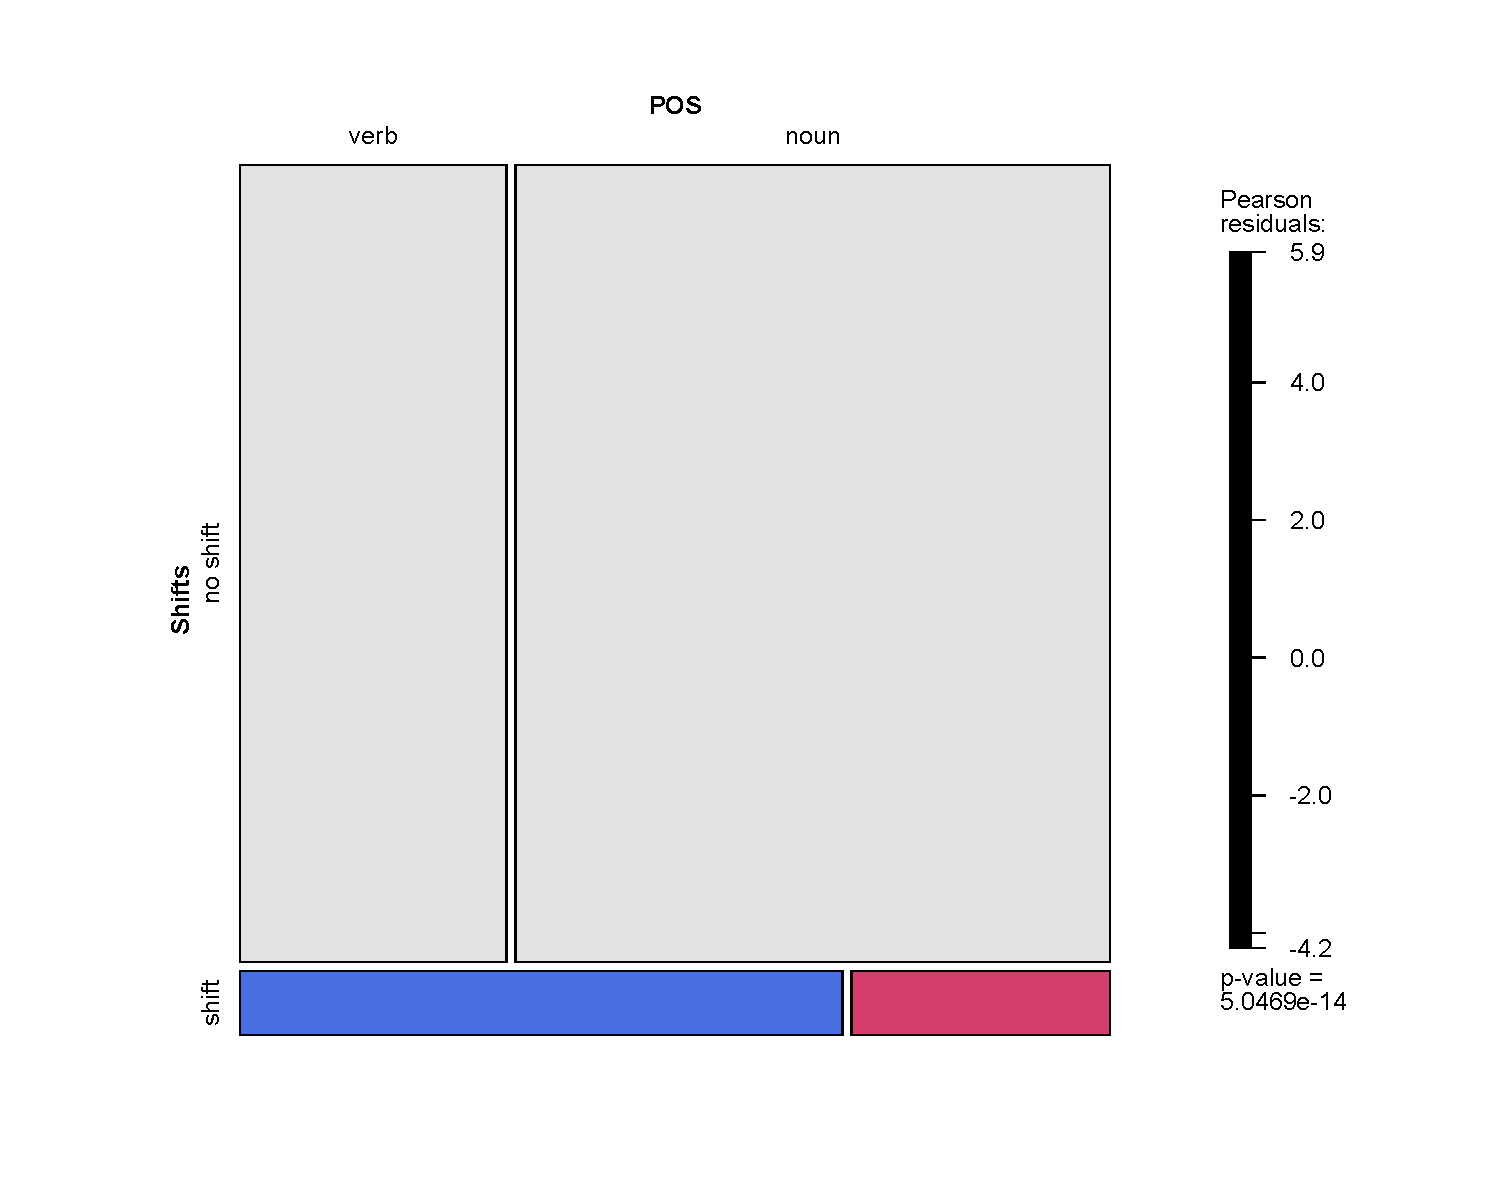
\includegraphics[width=0.7\textwidth]{figures/serbinaetal/serbinaetal1.pdf}
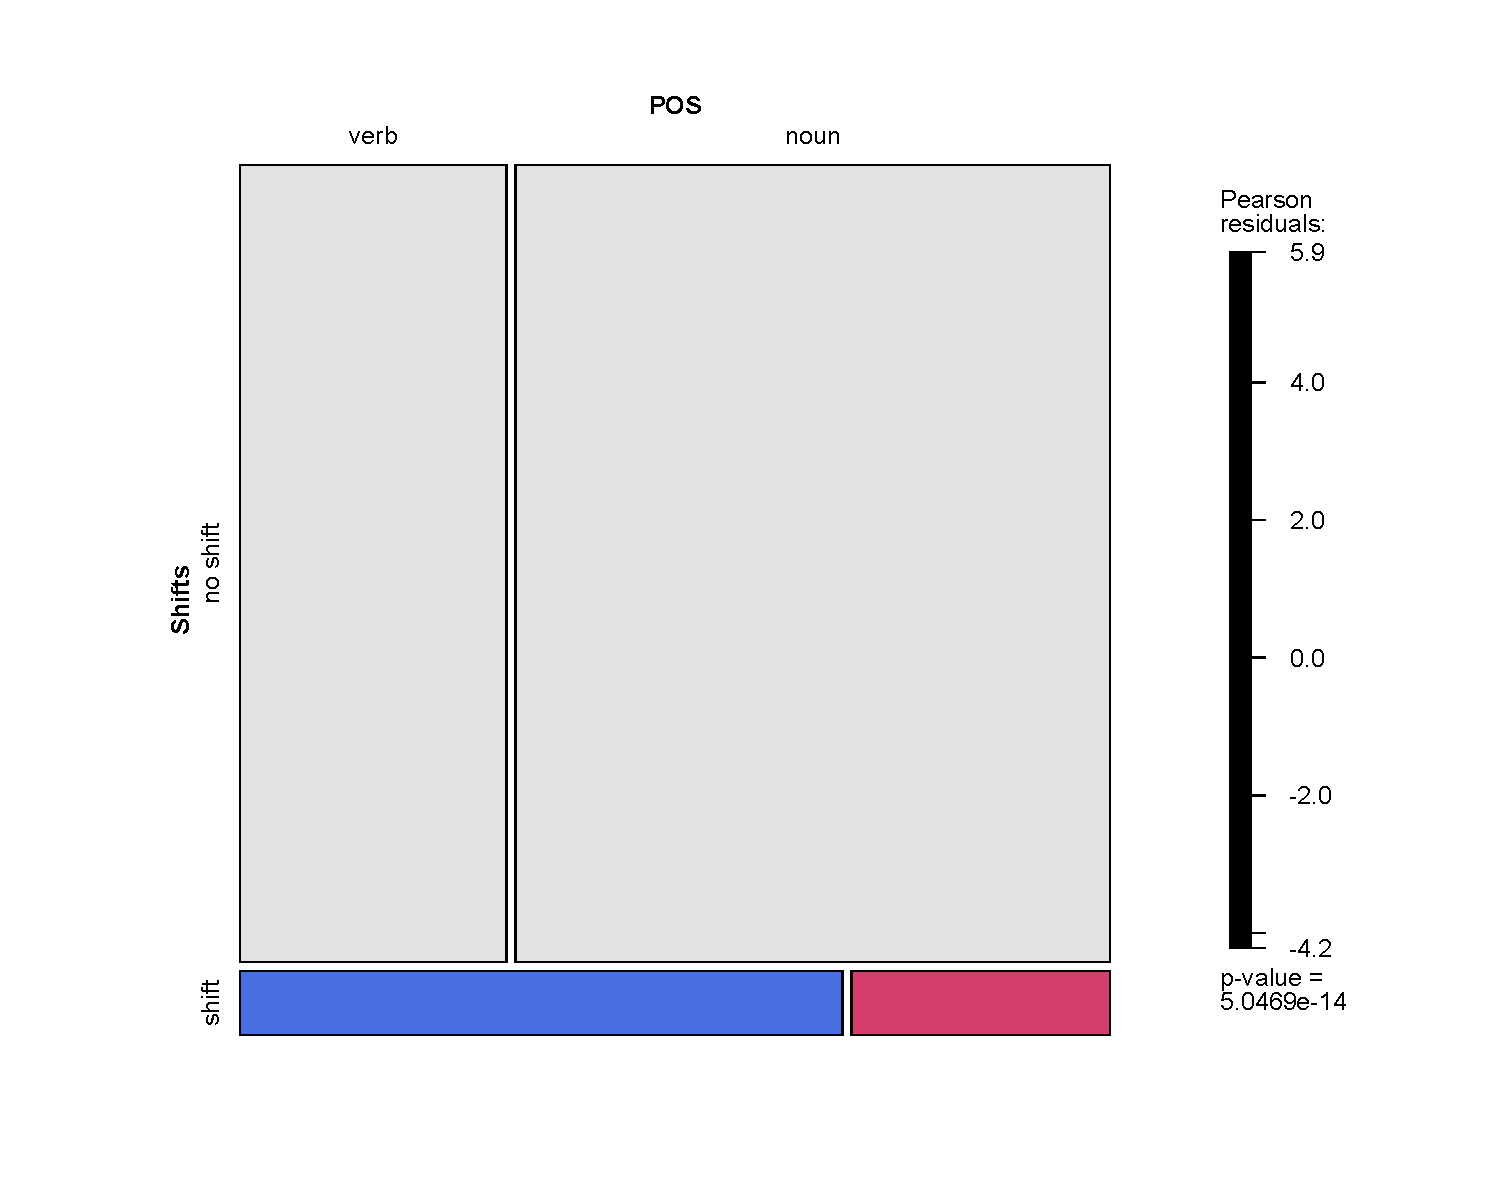
\includegraphics[width=0.7\textwidth]{figures/serbinaetal/serbinaetal1.pdf}
\caption{Mosaic plot for shifts from nouns and verbs in the final TT}
\label{serbinaetal:fig:2}
\end{figure}

This type of shift can be explained by a contrastive feature of the language pair English-\ili{German}. As reported in \sectref{serbinaetal:sec:2}, \ili{German} shows a tendency to be more nominal and certainly less verbal than English: thus the translations from English into \ili{German} may be influenced by the \isi{word class} distribution in the \ili{German} originals. The tendency to shift from a \isi{word class} that is less typical of the \isi{target language} can be linked to the translation property of normalization, according to which translators (over-)use the linguistic features that are associated with the \isi{target language} \citep[176]{Baker1996}. 

It is interesting to observe that most of the shifts from verbs to nouns were detected among the group of professional translators, who introduce this type of shift 26 times compared to only 12 instances among domain specialists. Due to the fact that the professionals translate on a regular basis, they can be expected to be more aware of contrastive differences within the language pair and try to adhere to the language norms of the \isi{target language}. The use of normalization is illustrated in \REF{serbinaetal:ex:5}:

\ea \label{serbinaetal:ex:5}
\textbf{EO:} [\ldots] a fact that $[$has confounded$]$\textsubscript{\textbf{Verb}} physicists. \\
\textbf{GTrans:} [\ldots] eine Tatsache, die Physiker $[$zum Grübeln bringt$]$\textsubscript{\textbf{PP}}. (KLTC PROBRAL GT3)
\z

In \REF{serbinaetal:ex:5}, the \isi{professional translator} shifts the verb \textit{confounded} to the more nominal (\textit{zum Grübeln bringen}, `make someone ponder $[$about$]$'). This shift, and similar shifts from the verb \textit{confound} in the English original to noun-verb combinations in \ili{German} translations, were considered to represent a shift from less to more nominal variants and were counted among `v-n' shifts.  
Participants also apply shifts in the opposite direction, namely from nouns to verbs, in 17 cases. This is also in line with Čulo et al.'s \citeyearpar{Culo2008} findings that shifts in \isi{word class} occur in both directions. They do, however, report differences in frequency with verb-noun shifts being clearly more frequent in the translation direction English to \ili{German}. Both \cite{Culo2008} and our own results illustrate the multifactorial character of translation due to which it is difficult to link empirical observations unequivocally with one particular source of explanation. 

\ea \label{serbinaetal:ex:6}
\textbf{EO:} the crumpled ball's $[$behavior$]$\textsubscript{\textbf{Noun}} [\ldots] \\
\textbf{GTrans:} wie sich die zusammengeknüllte Kugel $[$verhält$]$\textsubscript{\textbf{Verb}} (KLTC PROBRAL GP4)
\z

The translation in \REF{serbinaetal:ex:6} contains the verbal variant \textit{verhält} (`behaves'). This type of shift seems to counteract the tendency to adapt to the \isi{target language} norms and could be due to some kind of genuine \isi{source language} shining through \citep{Evert2017} not triggered by the immediate \isi{source language} textual environment but by the general activation of the \isi{source language} in the translator. It could, however, also support Steiner's \citeyearpar{Steiner2001Translations} assumption that the translator `unpacks' the complex variant (in \REF{serbinaetal:ex:6} a noun phrase expressing a process), i.e. links it to a simpler verbal version. The sentence pair in \REF{serbinaetal:ex:6}, and potentially other instances of n-v shifts, could not be interpreted as a direct confirmation of the literal hypothesis (\citealt{TirkkonenCondit2005}, \citealt{Schaeffer2013Shared}, \citealt{Halverson2015}): the analyzed target structure, which was produced as the first and final attempt by the participant GP4, is not primed by the aligned source text structure but rather in general by a structure common in the \isi{source language}.

The discussion of shifts between nouns and verbs should also consider the effect of individual lexical items in the source texts that are frequently shifted: 55 cases of shifts between the two main word classes correspond to 20 lexical items (5 distinct nouns that are translated as verbs and 15 verbs that are translated as nouns). Within the category noun-to-verb shifts, the noun \textit{crumpling} was frequently shifted to a verb (41.2\%, 7/17). The instance of \textit{crumpling} in the first version of the source text (see example \REF{serbinaetal:ex:7}) is classified as a noun based
on the definite article preceding it and the \textit{of}-genitive following it. This grammatical \isi{construction}, rather than the lexical item \textit{crumpling} itself, might be the reason for the shift in \REF{serbinaetal:ex:7}. 

\ea \label{serbinaetal:ex:7}
\textbf{EO:} After the $[$crumpling$]$\textsubscript{\textbf{Noun}} of a sheet of thin aluminized Mylar, the researchers placed it inside a cylinder. \\
\textbf{GTrans:} Die Forscher $[$knüllten$]$\textsubscript{\textbf{Verb}} hierzu ein Blatt aus dünnem aluminiertem Mylar [zusammen] und legten es in einen Zylinder. (KLTC PROBRAL GT5)
\z

Here, participant GT5 changed this noun to a \ili{German} verb, as did six other participants (87.5\%, 7/8). The remaining participant out of the eight who translated this version of the source text introduced a different shift, translating the noun with the nominalized infinitive \textit{das Zerknüllen} (`the crumpling'). While this translation is certainly more literal, this nominalization strategy  appears to be less frequent. We tested this assumption by querying the DWDS corpus, more specifically the core corpus of the 20th century \citepalias{BBAW2010}, for two nominalization strategies. The query for the sequence of the definite article \textit{das} followed by a noun ending in -\textit{en} returned 80,897 hits. To compare, the query for the definite article \textit{die} followed by a noun ending in -\textit{ung} returned 306,945 hits. Both queries do not target all the relevant cases, e.g. nouns preceded by demonstrative or personal pronouns, and potentially involve false hits, but these numbers give us an idea of the relative frequency of the nominalized infinitives. 

Among the shifts from verbs to nouns, the verb \textit{modeled} is shifted most frequently (18.4\%, 7/38). Example \ref{serbinaetal:ex:8} illustrates the most typical translation of this verb -- the noun \textit{Modell} (`model'). 

\ea \label{serbinaetal:ex:8}
\textbf{EO:} Scientists at the University of Chicago $[$modeled$]$\textsubscript{\textbf{Verb} }the relation between compression force and ball size.\\
\textbf{GTrans:} Wissenschaftler der Universität Chicago bauten im $[$Modell$]$\textsubscript{\textbf{Noun}} nach, wie sich die zum Zusammenpressen des Papierballs erforderliche Kraft im Verhältnis zu seiner Größe verhält. (KLTC PROBRAL GT1)
\z 

The verb \textit{modeled} is present in both versions of the source text. Thus this particular shift is present in slightly less than half of the translations (43.8\%, 7/16). However, it is interesting to observe that all of the seven instances can be found in the data of professional translators, while all eight domain specialists translated the verb using the \ili{German} verb \textit{modellieren} (`model'). This could be due to a meaning difference between the English verb and its \ili{German} \isi{cognate}, with the \ili{German} verb taking the more concrete meaning of shaping or sculpting. The fact that domain specialists tend to keep the verb could be arguably due to the use of loan translations in the hard sciences and thus re-introducing loan words to \ili{German}. However, this intuitive assumption should be further tested in future studies.

It is also worth considering the second most frequent shift from verbs to nouns (15.8\%, 6/38), namely from the infinitive \textit{compress}, as shown in \REF{serbinaetal:ex:9}. Since this particular instance of the verb occurs only in one of the two versions of the source text in our experiment, it was changed in 75\% of all cases (6/8). Two professional translators and two domain specialists chose to translate the infinitive \textit{compress} by a nominalized infinitive, \textit{Zusammendrücken}, whereas two other participants selected the noun \textit{Kompression}.  

\ea \label{serbinaetal:ex:9}
\textbf{EO:} Scientists at the University of Chicago modeled how the force required to $[$compress$]$\textsubscript{\textbf{Verb}} the ball relates to its size. \\
\textbf{GTrans:} Wissenschaftler der University of Chicago haben untersucht, in welchem Verhältnis die zum $[$Zusammendrücken$]$\textsubscript{\textbf{Noun}} des Papierballs erforderliche Kraft zu dessen Größe steht. (KLTC PROBRAL GT7) 
\z 

\tabref{serbinaetal:tab:4} also contains a shift from adverbs to prepositional phrases (see discussion of example \REF{serbinaetal:ex:5} above). This shift occurs 14 times in total but all of these cases can be traced back to the same lexical item in the English original, the adverb \textit{essentially}. While 14 participants translated this adverb into one of two fixed expressions in \ili{German}, namely \textit{im Wesentlichen} and \textit{im Grunde} (\textit{genommen}), two remaining participants opted for the adjectives \textit{grundsätzlich} and \textit{prinzipiell} in their translations. This English adverb potentially does not have a \isi{literal translation} equivalent in \ili{German}, so that a part of speech shift is very likely to take place. 

With respect to translation shifts, the analysis of English originals and their \ili{German} translations produced within our experiment has shown similar tendencies to those based on the CroCo Corpus, especially to \citet{Culo2008}. Participants frequently change ST verbs to TT nouns, thus selecting the \isi{word class} typical for the \isi{target language}. However, this investigation has also indicated that there are some differences in the frequency of the verb-noun shift depending on the group of participants, professional translators being more likely to change verbs into nouns. In the next section we will examine whether this type of shift is associated with particular phenomena during the \isi{translation process}.

% Section 5
\section{Process-based analysis}\label{serbinaetal:sec:5}
The process-based analysis is divided into two parts. In a first step, we use \isi{keystroke logging} data to enrich the product-based discussion by qualitatively analyzing intermediate versions of translation shifts between nouns and verbs. Secondly, we examine the amount of \isi{cognitive effort} associated with the translation of different parts of speech in general and with translation shifts in particular. 

\largerpage[-1]%longdistance
\subsection{Word class changes in the intermediate versions}\label{serbinaetal:sec:5:1}
Drawing on the intermediate translation versions recorded  via \isi{keystroke logging}, we analyzed the verb to noun and noun to verb shifts in more detail. Among the 38 verb to noun shifts, here was a single case in which the verb was translated to a noun, only to be shifted to another noun at a later point, thus producing a translation version chain verb-noun-noun. In contrast, three ST verbs were first translated into verbs before being changed into nouns at a later stage, as illustrated in \REF{serbinaetal:ex:10}:

\ea \label{serbinaetal:ex:10}
\textbf{EO:} Crumpling a sheet of paper seems simple and doesn't require much effort, but explaining $[$why the crumpled ball $[$behaves$]$\textsubscript{\textbf{Verb}} the way it does$]$\textsubscript{\textbf{Clause}} is another matter entirely. \\
\textbf{GTrans\_i:} Ein Blatt Papier zusammen zu knüllen, erscheint einfach und erfordert wenig Anstrengung, jedoch zu erklären, $[$warum das Papierknäuel sich so $[$verhält$]$\textsubscript{\textbf{Verb}}, wie es das tut$]$\textsubscript{\textbf{Clause}}, ist eine völlig andere Sache. \\
\textbf{GTrans\_f:} Ein Blatt Papier zusammen zu knüllen, erscheint einfach und erfordert wenig Anstrengung; $[$die $[$Verhaltensweise$]$\textsubscript{\textbf{Noun}} des Papierknäuels$]$\textsubscript{\textbf{NP}} zu erklären, ist dagegen eine völlig andere Sache. (KLTC PROBRAL GT7)
\z

First, the original ST verb \textit{behaves} is literally translated by the reflexive verb \textit{sich verhält} (reflexive pronoun + `behaves'). Both verbs are integrated into clauses and thus correspond to the grammatically simple variants. At this point, no translation shift at the level of word classes and no shift in \isi{grammatical complexity} has occurred. However, the verb \textit{sich verhält} is not present in the final TT. Instead, the verb \textit{behaves} corresponds to the noun \textit{Verhaltensweise} (`behavior'), which functions as the head of a noun phrase: the translator did not simply change the \isi{word class} but also shifted the level of \isi{grammatical complexity} from a simple to a more complex variant at the level of phrases (at the level of the clause the intermediate version is in fact more complex). Such a shift chain is in line with Tirkkonen-Condit's \citeyearpar{TirkkonenCondit2005} claim, according to which the first translation solution is likely to be literal, but can be later revised if deemed necessary (\citealt{TirkkonenCondit2008} as well as \citealt{Schaeffer2013Shared}, \citealt{Halverson2015}).

Among the seventeen shifts in the opposite direction, i.e. from ST nouns to verbs in the final TTs, there are one instance of the chain `noun-noun-verb', two instances of the chain `noun-verb-verb' and even one instance, shown in \REF{serbinaetal:ex:11}, involving a longer chain consisting of a noun and three verbs:

\ea \label{serbinaetal:ex:11}
\textbf{EO:} $[$After the $[$crumpling$]$\textsubscript{\textbf{Noun}} of a sheet of thin aluminized Mylar$]$\textsubscript{\textbf{PP}}, the researchers placed it inside a cylinder. \\
\textbf{GTrans\_i1:} $[$Nachdem sie ein dünnes Blatt aluminiumbeschichtetes Mylar $[$verkrumpelt$]$\textsubscript{\textbf{Verb}} hatten$]$\textsubscript{\textbf{Clause}}, gaben sie es in einen Zylinder. \\
\textbf{GTrans\_i2:} $[$Nachdem sie ein dünnes Blatt aluminiumbeschichtetes Mylar $[$verknäuelt$]$\textsubscript{\textbf{Verb}} hatten$]$\textsubscript{\textbf{Clause}}, gaben sie es in einen Zylinder. \\
\textbf{GTrans\_f:} $[$Nachdem sie ein dünnes Blatt aluminiumbeschichtetes Mylar $[$verknittert$]$\textsubscript{\textbf{Verb}} hatten$]$\textsubscript{\textbf{Clause}}, gaben sie es in einen Zylinder. (KLTC PROBRAL GT3)
\z


\largerpage[-1]%longdistance
Here the original noun \textit{crumpling} in the prepositional phrase was shifted directly to a verb. This change led to a reduction in \isi{grammatical complexity}. In the subsequent intermediate versions, the translator made lexical changes without further altering the grammatical structure of the sentence. This suggests that the effort these changes cause is primarily due to lexical search in the production phase of the translation rather than \isi{cognitive effort} caused by the grammatical structure of the source text segment. Otherwise, a wider section of the unfolding target text might have been affected by the changes during the \isi{translation process}. 

Changes in \isi{word class} seem to be fairly straightforward for the participants. Only 8 out of the 55 cases of shifts discussed in this section, i.e. 14.5\%, actually involved more than one step during translating. 

While it would be interesting to include these more complex chains of part-of-speech shifts in the analysis of cognitive processing, such an analysis is not possible at the present stage due to a low number of shifts in the intermediate versions found in our data. This investigation should be performed when the keystroke logged translation corpus is extended to include data from further experiments. Once the number of the intermediate versions and the direction of such shifts are added into the regression models, the estimates for the analyzed eye-tracking measures can potentially change. We would expect that modifications on the lexical level, leading to such chains as `n-n-n', already result in more \isi{cognitive effort}, reflected in more and longer fixations on the corresponding ST word simply due to additional processing associated with search for the right lexical item. In addition, chains of the types discussed in this section are likely to result in further increase of cognitive processing due to changes of grammatical structure. However, such lexical and grammatical changes may be also made `silently' without additional fixations on the source text, but rather after (multiple) re-reading of the intermediate versions of the target text. Here, an eye-tracking analysis of the target text should provide us with additional insights. Due to the technical problem of continuously changing screen contents while producing the translation (and recording eye movements), currently it is not possible to analyze specific areas in the target text window. 


We now turn to the eye-tracking data to understand the effect of translating the different parts of speech -- involving shifts or not -- on \isi{cognitive effort}. 

\subsection{Eye-tracking data}\label{serbinaetal:sec:5:2}
As mentioned in \sectref{serbinaetal:sec:2}, the word classes of verbs and nouns can be linked to clausal and nominal ways of expressing meaning. Since at least the nominal variants of nouns expressing processes (see \citealt{Fontaine2017}) are considered more complex, we would expect the processing of nouns to involve more \isi{cognitive effort} than the processing of verbs. Moreover, we assume that shifts from simpler to more complex variants, i.e. from verbs to nouns, are cognitively more effortful than shifts in the opposite direction. These hypotheses were tested using the eye-tracking data, operationalizing \isi{cognitive effort} through the measures of \isi{total fixation duration} and \isi{fixation count} \citep{Holmqvist2011}. As cumulative measures, these are fairly general, potentially capturing various phenomena such as lexical access, preparing for the translation in addition to \isi{grammatical complexity}. As it does not appear possible to disentangle these factors in a principled way in the given experiment design, the cumulative measures appear to be a plausible first step. Future work includes another experiment involving a more controlled setting which will allow to analyze more targeted eye-tracking measures. For the analyses of the eye-tracking data, we consider nouns that were shifted to verbs, verbs that were shifted to nouns, as well as random samples of 30 nouns and 30 verbs (see \sectref{serbinaetal:sec:3})

\newpage 
Boxplots in \figref{serbinaetal:fig:3} show \isi{total fixation duration} and \isi{fixation count} on the ST nouns and verbs.\footnote{The data with no shifts includes one ST verb and three ST nouns with no fixations. Since the words were translated, it is unlikely that they were not processed at all. Therefore, these cases are treated as NAs (not available) rather than zero values.} They indicate that, contrary to our first assumption, verbs in general are fixated slightly longer and more often than nouns. However, it is important to keep in mind that this representation averages over eye movements on all nouns and verbs under analysis, i.e. with and without shifts. 

\begin{figure}[t]
	\begin{subfigure}{.47\textwidth}
  	\centering
  	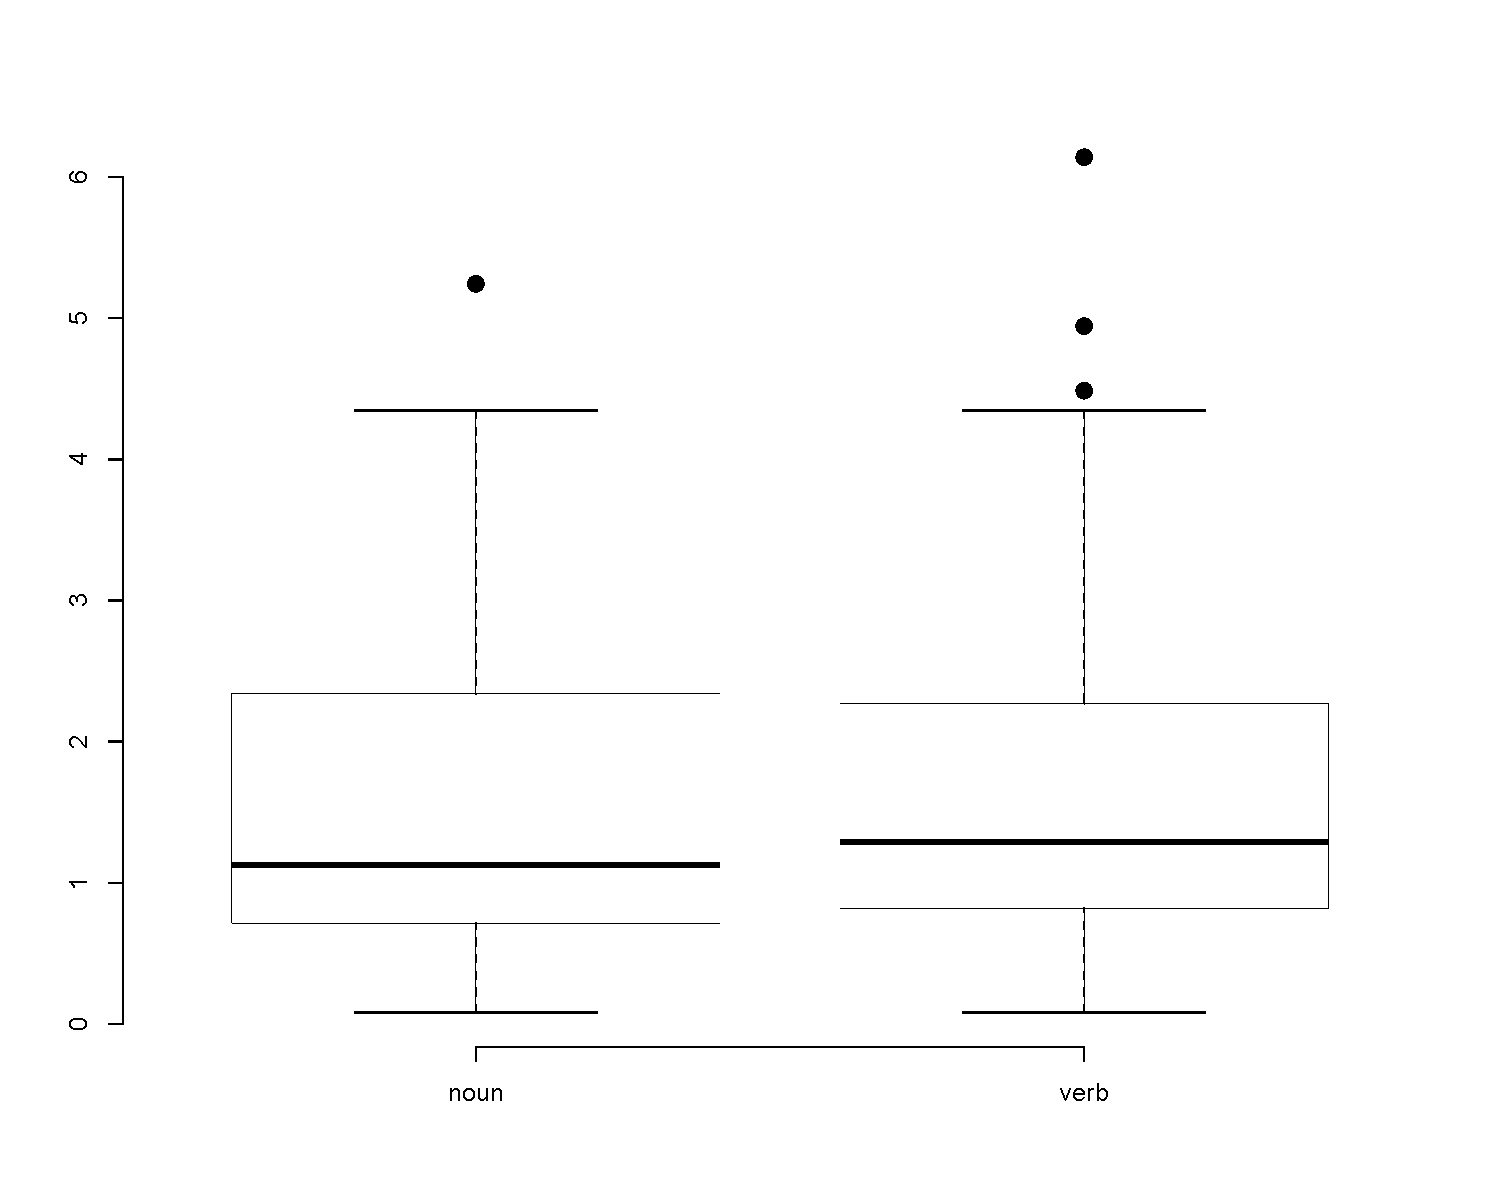
\includegraphics[width=\linewidth]{figures/serbinaetal/serbinaetal2.pdf}
	\end{subfigure}
    \begin{subfigure}{.47\textwidth}
  	\centering
  	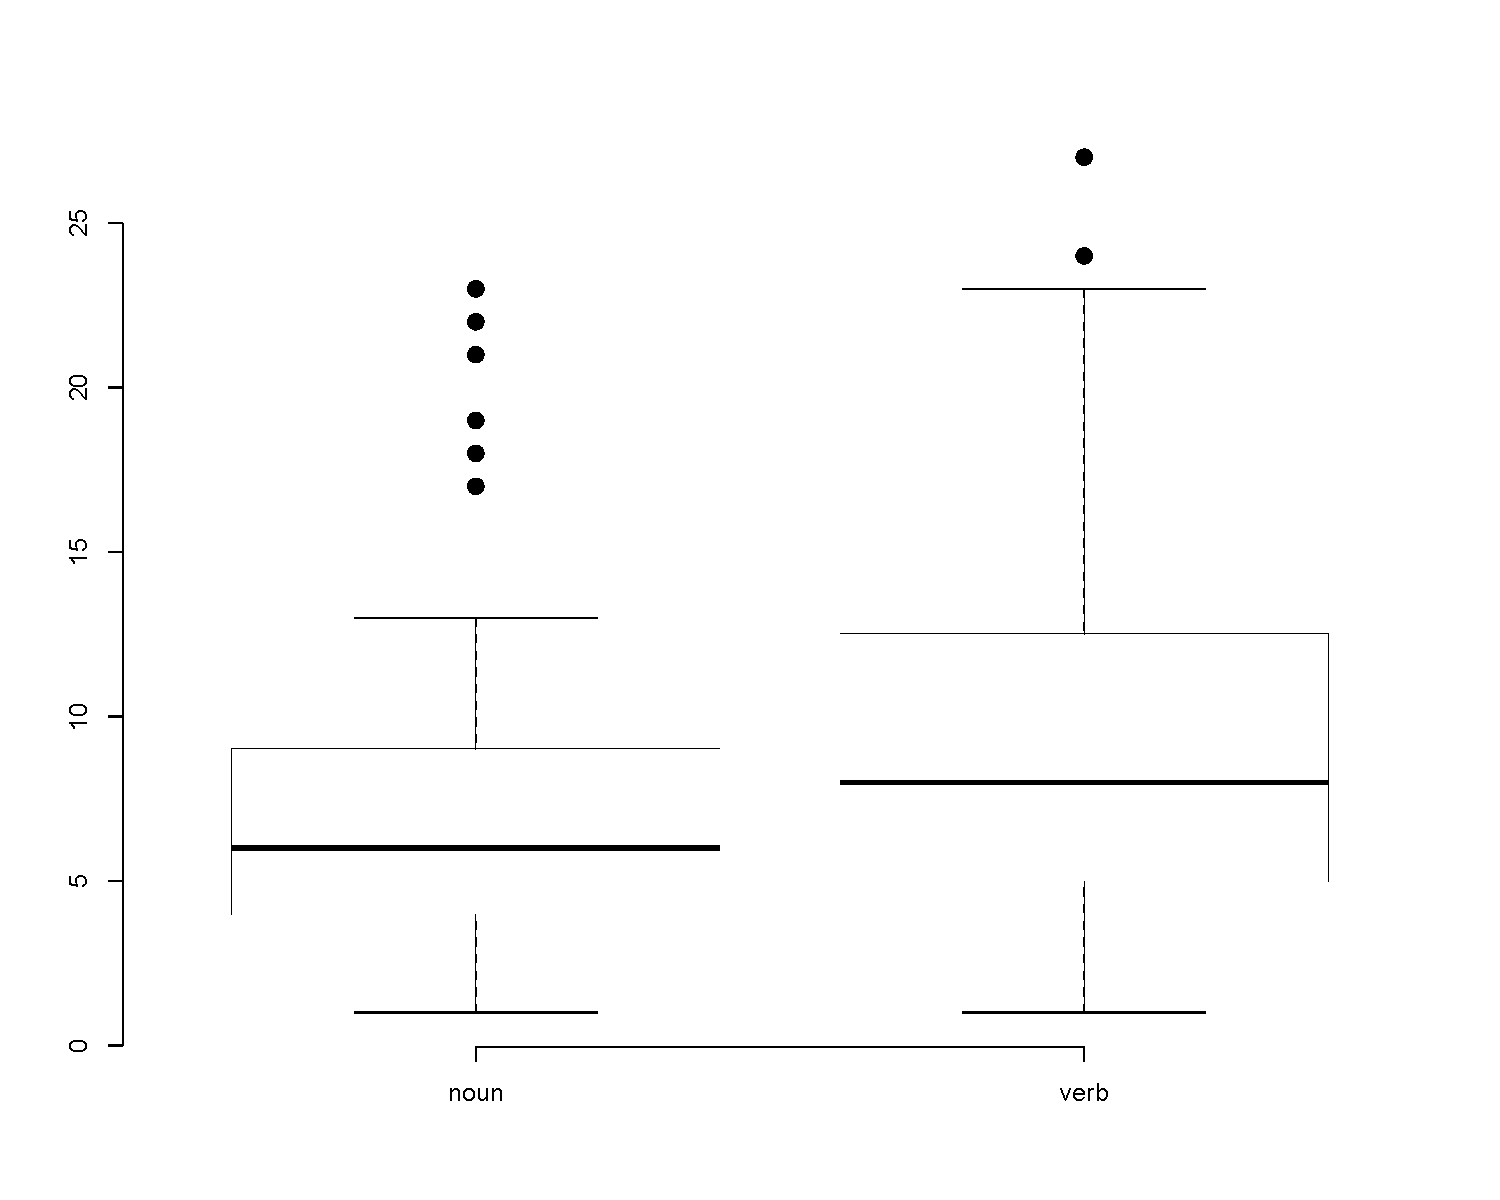
\includegraphics[width=\linewidth]{figures/serbinaetal/serbinaetal3.pdf}
	\end{subfigure}
\caption{Total fixation duration (left) and fixation count (right) for nouns and verbs}
\label{serbinaetal:fig:3}
\end{figure}
  
\begin{figure}[t]
	\begin{subfigure}{.47\textwidth}
  	\centering
  	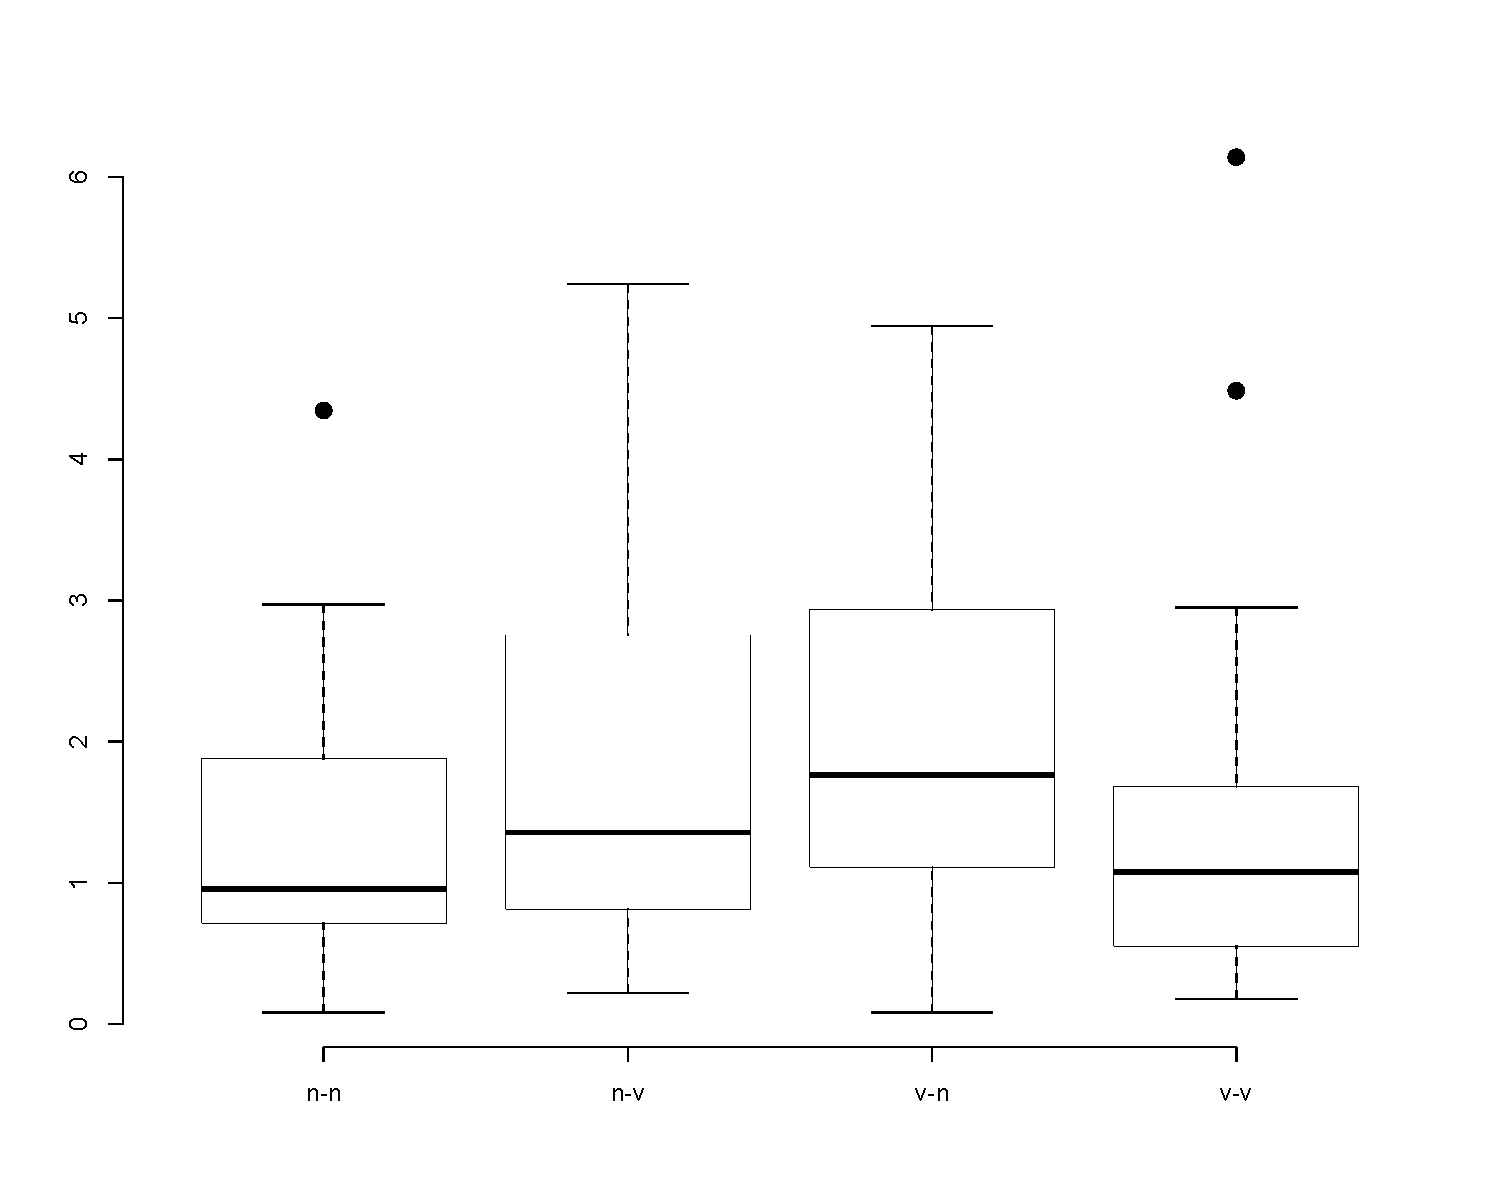
\includegraphics[width=\linewidth]{figures/serbinaetal/serbinaetal4.pdf}
	\end{subfigure}
    \begin{subfigure}{.47\textwidth}
  	\centering
  	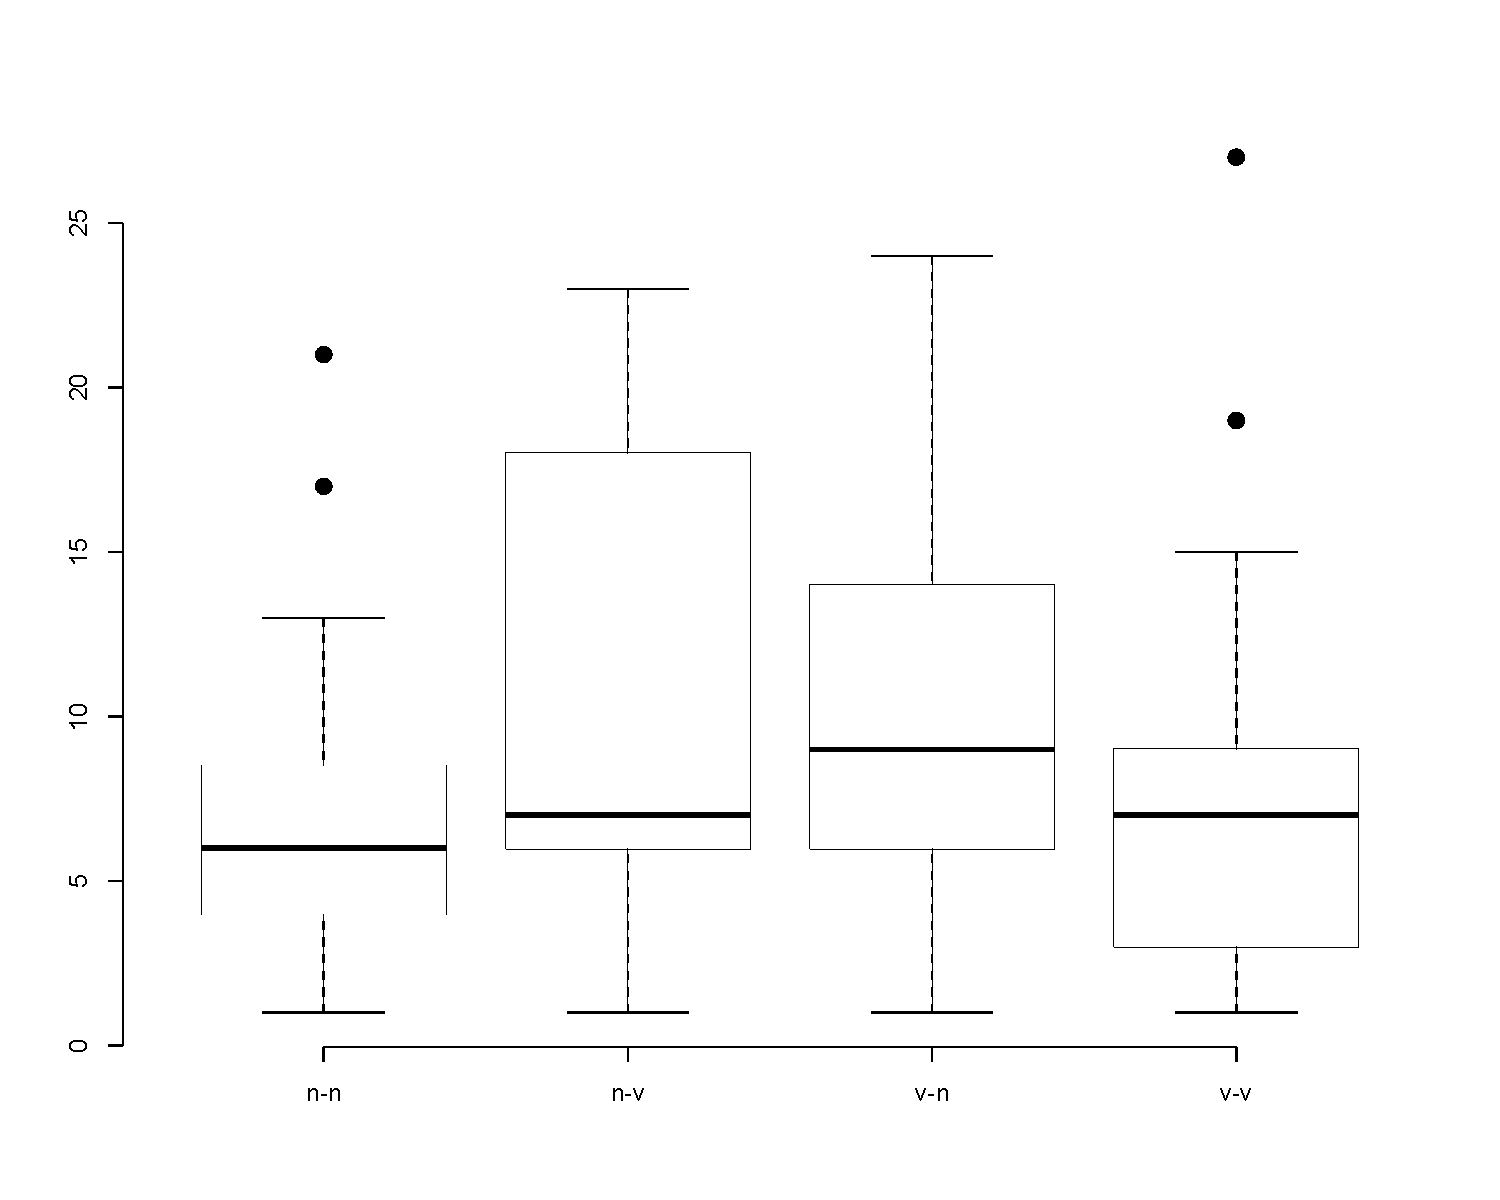
\includegraphics[width=\linewidth]{figures/serbinaetal/serbinaetal5.pdf}
	\end{subfigure}
\caption{Total fixation duration (left) and fixation count (right) for noun-verb and verb-noun shifts}
\label{serbinaetal:fig:4}
\end{figure}

\figref{serbinaetal:fig:4} presents a more differentiated picture, showing the descriptive statistics for the four types of alignment pairs: 1) ST nouns that correspond to TT nouns, 2) ST nouns that were changed to TT verbs, 3) ST verbs that were shifted to TT nouns and 4) ST verbs that were translated into TT verbs. Comparing the data with no shifts, we can see that the median for the fourth group involving verbs is very similar to that for the first group consisting of noun-noun pairs. Also the ST nouns that are shifted to verbs (group 2) has similar eye-tracking values. However, ST verbs that correspond to nouns in the TT (group 3) are characterized by longer \isi{total fixation duration} and more fixations. 

To analyze whether this difference is statistically significant and to account for additional sources of variation, two mixed-effects regression models were calculated using the lme4 R package \citep{Bates2015}. For the dependent variable of ``Total Fixation Duration'', a linear mixed-effects model was selected. To approximate a normal distribution of this variable, it was log-transformed. Since ``Fixation Count'' represents count data, we chose a Poisson mixed-effects regression to model this eye-tracking value. The nominal independent variable labeled ``Changes'' contains four levels corresponding to the four types of alignment pairs discussed above. The model includes the confounding factor ``Group (of participants)'' to account for the fact that the target texts were produced by either professional translators or domain specialists, and ``Length (of the ST item in characters)'' as another control variable. We also added random intercepts for individual experiment participants and different source text words, as in some cases the analyzed word classes were realized by the same lexical items. 

\tabref{serbinaetal:tab:6} summarizes the results of the fixed effects for the linear mixed-effects regression model with ``Total Fixation Duration'' as the dependent variable. The results of the fixed effects for the Poisson mixed-effects regression model with ``Fixation Count'' as the dependent variable are presented in \tabref{serbinaetal:tab:7}. Statistical significance of the variable ``Changes'' was tested using a likelihood ratio test comparing the models with and without this independent variable. Moreover, the significance of simple effects, presented in the following table, was computed using the \textit{lmerTest} package \citep{Kuznetsova2016}. 

\begin{table}
\begin{tabularx}{\textwidth}{Xd{4}d{4}d{3}d{3}d{3}} 
\lsptoprule
				& \multicolumn{1}{c}{Estimate} 	& \multicolumn{1}{c}{Std. Error} 	& \multicolumn{1}{c}{df} 	& \multicolumn{1}{c}{$z$ value} & \multicolumn{1}{c}{Pr (> $|t|$)} 	\\ \midrule
(Intercept) 	& -0.431 	& 0.378 		& 47.66 & -1.14 	& 0.26			\\
Changes n-v 	& 0.371 	& 0.281 		& 47.55 & 1.32 		& 0.19			\\
Changes v-n 	& 0.49 		& 0.214 		& 51.72 & 2.29 		& 0.03			\\
Changes v-v 	& 0.099 	& 0.22 			& 56.72 & 0.45 		& 0.66			\\
TranslatorGroup & 0.123 	& 0.32 			& 12.98 & 0.39 		& 0.71			\\
STWordLength 	& 0.04 		& 0.04 			& 41.58 & 1.01 		& 0.32			\\
\lspbottomrule
\end{tabularx}
\caption{Linear mixed-effects model, ``Total Fixation Duration'' as dependent variable}
\label{serbinaetal:tab:6}
\end{table}

\begin{table}
\begin{tabularx}{\textwidth}{Xd{3}d{3}d{3}S[table-format=>1.2e+1]} 
\lsptoprule
				& \multicolumn{1}{c}{Estimate} 	& \multicolumn{1}{c}{Std. Error} 	& \multicolumn{1}{c}{$z$ value} 	& \multicolumn{1}{c}{Pr (> $|t|$)}	\\ \midrule
(Intercept) 	& 1.62 		& 0.28 			& 5.85 		& <.001		\\
Changes n-v 	& 0.38 		& 0.17 			& 2.2 		& 0.03			\\
Changes v-n 	& 0.4 		& 0.14 			& 2.84 		& 0.005			\\
Changes v-v 	& 0.12 		& 0.15 			& 0.85 		& 0.4    		\\
TranslatorGroup & 0.03 		& 0.22 			& 0.14 		& 0.89    		\\
STWordLength 	& 0.03 		& 0.03 			& 0.99 		& 0.32  		\\
\lspbottomrule
\end{tabularx}
\caption{Poisson mixed-effects model, ``Fixation Count'' as dependent variable}
\label{serbinaetal:tab:7}
\end{table}

  
Examining the estimates for the four types of possible alignment pairs, we can see that the shifts from verbs to nouns lead to a larger increase in \isi{total fixation duration}. This simple effect of the level of the variable ``Changes'' is significant ($p=0.03$). Moreover, both types of shifts, i.e. from verbs to nouns ($p=0.005$) as well as from nouns to verbs ($p=0.03$), are associated with significantly more fixations on the corresponding ST verbs and nouns, as compared to nouns and verbs that are translated by the same word classes. The overall effect of the variable ``Changes'' reaches the conventional level of significance of 0.05 only in the Poisson regression model with ``Fixation Count'' as the dependent variable ($p=0.09$ for ``Total Fixation Duration'' as the function of ``Changes''; $p=0.01$ for ``Fixation Count'' as the function of ``Changes''). 

As pointed out before, our current analysis is based on cumulative eye-tracking measures, which may also include at least preparation of the translation. So, the increase in number and the total length of fixations for the verbs shifted to nouns could possibly be related to the added effort caused by the change into a noun. This is in line with our second assumption of increased cognitive processing associated with shifts to more complex structures. The potentially more effortful production of a more complex segment appears to be a viable explanation for the fact that the translation products still contain a certain amount of noun-verb shifts, although the contrastive differences in the distribution of nouns and verbs in English and \ili{German} would predict an increase in the number of nouns in the translations. At the same time, we should consider that nouns shifted into verbs are fixated at least more often, if not (significantly) longer. Thus, it appears that the increased \isi{cognitive effort} could be associated with a \textit{change} in \isi{grammatical complexity} during the process of translation, rather than with the \textit{level} of complexity in the source or target text segment. However, it should be kept in mind that word classes provide only an indirect link to phrasal vs. clausal complexity discussed in \sectref{serbinaetal:sec:2}. Further information on grammatical context is required to enrich the performed analysis. Moreover, the cumulative eye-tracking measures used in this study may mask a more fine-grained effect of the inherent complexity of nominal versus verbal expressions. Future work addressing such delicate phenomena will also have to include separating the effect of lexical considerations from dealing with \isi{grammatical complexity}.

% Section 6
\section{Conclusion and outlook}\label{serbinaetal:sec:6} 
We hope to have shown that shifts from verbs to nouns account for the majority of shifts between the main word classes in our data containing translations from English into \ili{German}. Analysis of the \isi{keystroke logging} data showed that shifts in \isi{word class} tend to be implemented in one step. This result is in line with a previous study by \citet{Alves.2014} based on the same data,\footnote{The translation experiment conducted within the project \textit{PROBRAL} (see \sectref{serbinaetal:sec:3} for more details) was performed for two language pairs, namely for English-\ili{German} and English-\ili{Portuguese}. While the present study considers all the data for the translation direction English-\ili{German}, the study by \citet{Alves.2014} concentrates on the translations of one stimulus included into the ST but takes into account both \ili{German} and \ili{Portuguese} translations.}  which showed that over a half of all experiment participants produced just one translation solution for the analyzed ST passage. Moreover, the majority of participants did not change the initial level of \isi{grammatical complexity} associated with their proposed translation, even if they did change their first translation version. The authors conclude that translators are likely to decide on the grammatical structure before they produce the first translation version, and, if they modify this version at all, then the changes tend to be lexical rather than grammatical \citet[39]{Alves.2014} . Although it is possible that producing one translation is accompanied by longer processing periods, it is more plausible to conclude that one-step translations are not linked to increased effort. This assumption is corroborated by another finding reported in \citet{Alves.2014}. The authors have shown that the three translations that do involve shifts in \isi{grammatical complexity} between different versions (shifts between intermediate and final translation versions) appear to involve more \isi{cognitive effort} \citet[40]{Alves.2014} . To test this assumption further, our next step should be to include the shifts in \isi{word class} present in the intermediate versions into the analysis of cognitive processing associated with translation of nouns and verbs. Another interesting aspect for closer investigation is the analysis of intermediate versions for shifts in \isi{word class} where the aligned source and target texts do not indicate a shift \citep{Niemietz2014}.

The regression models indicated some statistical association between the types of alignment pairs and the eye-tracking measures of \isi{total fixation duration} and \isi{fixation count}. There appears to be a tendency to fixate the verbs that correspond to nouns in the final translations longer and more often. Moreover, also the nouns that correspond to verbs in the final translations are fixated more often. In fact, the overall effect of the variable ``Changes'' is significant for the model operationalizing \isi{cognitive effort} in terms of ``Fixation Count''. These initial findings suggest that changing \isi{grammatical complexity} in general might be effortful.

In this paper, identification and linguistic annotation of the relevant intermediate versions was performed manually for the experiment data examined. Automatic tokenization and part of speech annotation of the \isi{keystroke logging} data allows for processing of more data points necessary for more detailed statistical analyses. Such automatic part of speech annotation of intermediate versions has been recently developed \citep{Serbina2015Part} but is, at the moment, applicable only to the keystrokes collected with Translog II. Once it is extended to allow analyses of the Translog 2006 files, such as the ones generated in this translation experiment, the process-based investigations should be repeated taking into account not only random samples but all alignment pairs of the types `noun-noun' and `verb-verb', since these can also be characterized by intermediate versions. Even without such advanced methods, this paper has already shown the kind of more detailed test of long-held assumptions that a combined product and process-based analysis of linguistic features can yield. 

\section*{Acknowledgement}
We would like to thank Arndt Heilmann for the valuable discussions of the paper. The authors gratefully acknowledge support of the \ili{German} Research Foundation (DFG) project \textsc{Tricklet} (Translation Research in Corpora, Keystroke Logging and Eye Tracking), research grant no. NE1822/2-1, and the RWTH HumTec Boost Fund Project e-cosmos by the Excellence Initiative of the \ili{German} State and Federal Governments.

\newpage 
\sloppy
\printbibliography[heading=subbibliography,notkeyword=this]
\end{document}
